\documentclass[9pt,twocolumn,twoside]{../../styles/osajnl}
\usepackage{fancyvrb}
\journal{i524} 

\usepackage{graphicx}
\usepackage{listings}
\usepackage{color}

\definecolor{dkgreen}{rgb}{0,0.6,0}
\definecolor{gray}{rgb}{0.5,0.5,0.5}
\definecolor{mauve}{rgb}{0.58,0,0.82}

\lstset{frame=tb,
  aboveskip=3mm,
  belowskip=3mm,
  showstringspaces=false,
  columns=flexible,
  basicstyle={\small\ttfamily},
  numbers=none,
  numberstyle=\tiny\color{gray},
  keywordstyle=\color{blue},
  commentstyle=\color{dkgreen},
  stringstyle=\color{mauve},
  breaklines=true,
  breakatwhitespace=true,
  tabsize=3
}

\title{Deployment of Vehicle Detection application on Chameleon clouds}

\author[1,*]{Abhishek Naik}
\author[2,*]{Shree Govind Mishra}

\affil[1]{School of Informatics and Computing, Bloomington, IN 47408, U.S.A.}
\affil[2]{School of Informatics and Computing, Bloomington, IN 47408, U.S.A.}
\affil[*]{Corresponding authors: absnaik810@gmail.com, shremish@indiana.edu}

\dates{project-001, \today}

\ociscodes{Vehicle detection, Ansible, Cloudmesh, OpenCV, Haar Cascades, Cloud, I524}

\doi{Report:
  \url{https://github.com/cloudmesh/sp17-i524/tree/master/project/S17-IR-P010/report/report.pdf}\\
Code: \url{https://github.com/cloudmesh/cloudmesh.vehicle}}

\begin{abstract}
This project focuses on the deployment of Vehicle Detection
application on multiple Chameleon clouds using Ansible playbook.  It
also focuses on the benchmarking of the deployment results and its
analysis.\newline
\end{abstract}

\setboolean{displaycopyright}{true}

\begin{document}

\maketitle

\section{Introduction}

Vehicle Detection forms an integral part of the development of new
technologies like fully self-driving cars, etc.  One of the techniques
to perform such detection is by using Haar Cascades \cite{haar-cascade}.  This
technique has been applied to vehicle detection by creating a
haar-cascade cars.xml file which has been trained using 526 rear-end
images of cars.  In this project, we would be extending this vehicle
detection approach to enable it to run on multiple clouds.  This
deployment would initially be done on the localhost, followed by
deployment on the cloud.  Cloudmesh client would be used
for cloud management and Ansible scripts would be used for software
stack deployment.  The vehicle detection application would then run remotely onto the clouds.  The result would be an image (a .jpg file) with all the vehicles in it detected with a red rectangle around it and sent back to the local host.  Appropriate benchmarking would be carried out at
each iteration using some benchmarking technique.  

\section{Requirements}
The requirement was to deploy the Vehicle detection application onto the cloud's Virtual Machines (VMs).  The processing, which included detection of vehicles by drawing a red rectangle around them, had to be carried out on the cloud VMs.  The output image that was generated had to be then resent back to the local machine.  

\section{Software stack}
For this project, we have used the following software/applications:

\begin{itemize}

\item[$\bullet$] Ansible \cite{Ansible}: \\
Ansible is an open source platform that is used for automation.
Configuration management, task automation and application deployment
can be carried out using Ansible.  In our project, we have used
Ansible to manage the configuration and automate the deployment of the
software stack onto the clouds.  We run Ansible scripts via localhost
entering the IP addresses of the cloud's VMs and
the software/applications are installed in those VMs.  Thus, we are
using Ansible to orchestrate the software deployment via playbooks
using the inventory.txt file containing the IP addresses.

Ansible forms connections to our cloud VMs and then pushes 'Ansible modules', which are nothing but small programs, to them.  Ansible executes these modules and then removes them upon completion.  Ansible thus helped us in lightweight development, in the sense that other than an editor and the terminal, it did not require any other components to be installed.  Although we used SSH keys for the connections and with Ansible, Ansible also supports the use of passwords.  

\item[$\bullet$] Cloudmesh client \cite{github-cloudmesh-client}: \\
Cloudmesh is basically used for cloud VM management.  It provides
easy access to different cloud environments via a command shell and
command line.  In our project, we have used Cloudmesh client for
dynamic management of the cloud VMs.  Cloudmesh client enabled us to boot up the virtual machines on the clouds, assign floating IPs, etc.  Thus, we have used it to carry about these activities as well as add
our SSH keys to a local database and then SSH to the remote VMs on
the clouds using various cloudmesh client commands and utilities.  

\item[$\bullet$] Python \cite{Python}: \\
Python is an object oriented, high level programming language.  It is
an interpreted language and provides built-in data structures with
dynamic typing and binding.  It has an easy and simple yet intuitive
syntax.  In our project, we are using Python (and Pip \cite{Pip}) for
the installation and management of software written in Python.

\item[$\bullet$] Git \cite{Git}: \\
Git is a version control system that can be used for tracking and
change management when multiple people are involved in a project.  It
helps control and coordinate the working among a group of people.  We
have used Git to manage our work within our team.  It has helped us by
providing a central place wherein we could commit our work and make it
easily accessible to others.  Also, the Vehicle Detection Application
(outlined below) application that we are using in our project has been
developed and hosted on Github by the creator Andrews Sobral.  We have
forked his repository and using his application for the detection of
vehicles.

\item[$\bullet$] OpenCV \cite{OpenCV}: \\
OpenCV is a collection (library) of various functions used to execute
computer vision related applications.  The Vehicle Detection
Application runs on OpenCV.  OpenCV includes both, a trainer as well
as a detector.  It also has many pre-trained classifiers.  We are
using the Haar classifier \cite{haar-cascade}.

\item[$\bullet$] Vehicle Detection Application \cite{vehicle-detection-application}: \\
The Vehicle Detection Application has been developed by Andrews
Sobral.  It basically uses a haar-cascade cars.xml for vehicle
detection.  The haar-cascade was trained using 526 rear-end images of
the cars.  The video size used is 360x240 pixels.  In our project, we
are running this application on the clouds.

\item[$\bullet$] Bash script \cite{Bash-script}:\\
Bash typically helps us in the automatic execution of various Linux commands by creating a .sh file.  We have used a file myScript.sh in order to carry out the benchmarking of the project.  It should be noted that once a shell script is created, appropriate permissions (or privileges) must be set so that it is executable.  We call the ansible script to be executed within this shell script.  We can thus say that the Bash script is the starting point of our project - we just have to run this script and then the software stack including the Vehicle detection application would be deployed, the application would be run and the generated image file would be rerouted to our local machine.  In order to carry out benchmarking, we just did a minor modification to this routine (edited the inventory.txt file).

\end{itemize}

\section{Deployment}

For successful project deployment, the first step was gaining access
to the clouds.  Cloudmesh client was used for gaining this access.  In
order to set up this cloudmesh client, we had to configure the
cloudmesh.yml file with our credentials and other details.  We mainly
used Chameleon clouds in our project so we only edited the
cloudmesh.yml file parts that corresponded to chameleon clouds.  If we
were to use Jetstream, we would have required to edit the Jetstream
part as well.  We had to edit the values in such a way as to ensure
that the info command did not yield any To Be Decided (TBD) values.
In case it did, then it meant that there were possibly some errors and
we had to revisit the cloudmesh.yml file and correct those.  If there
were no TBD values at all, then it meant that we were good and could
now access the clouds.  Once we had access to the clouds, we booted a
VM and then assigned a floating IP to it.  Post this, we used the SSH
command to log in into the VM.  Once we were within the VM, we could
use it as a normal local Ubuntu machine.  Although we didn't require
it in this project, cloudmesh also provided the functionality to use a
different image on the cloud VMs.

When we need a new VM, we simply booted a new VM and assigned a new
floating IP address to it.  This resulted in allocation of a new VM
which we could then use as a new additionL machine.  By proper set up
in the Ansible scripts, one of these machines could be used as a
master and the other one(s) as slaves, if there is a need in some
project.

The second step was the identification of the software stack that
would be required.  In order to understand this, we first deployed the
software and application on the local machines and then on the
clouds.  This step helped us understand the software needed as well
as the dependencies amongst them.  Once we identified the software,
we developed an ansible script to deploy the software and
applications dynamically in an automated way.

Ansible is an open source automation platform.  It mainly uses .yml
files for its working.  The file 'inventory.txt' contains the details
of the hosts (their IP addresses) wherein the software stack is to be
installed.  Similarly, we can also mention the ansible username in
this file.  Thus, in our case, the entry in the inventory.txt file is
as below:

\begin{lstlisting}
 129.114.110.83 ansible_ssh_user=cc
\end{lstlisting}  
	
The 'playbook.yml' file lists the hosts, variables and the roles.  The
hosts contains the details of the machine where the software are to
be installed.  The variables section lists the variables that are
being used elsewhere, for e.g., '\texttt{dwnld\_dr}' denoting the download
directory.  The advantage of using variables is that the values do not
need to be hard coded and thus they can be changed everywhere with a
minor update.  The roles section lists the various software that need
to be installed, in order.  In our case, the entry of the playbook.yml
file is as below:

\begin{lstlisting}
	---
	- hosts: all
          vars:
	    dwnld_dr: ~/downloads}
	    ocv_ver: 2.4.13.2}
	    repository: {{ repository }}
	    tmp: /tmp/vehicledetection
          roles:
	    - git
	    - python
	    - upgrade
	    - opencv
	    - vehicledetection
\end{lstlisting}
                
The 'roles' directory contains the details about all the software
that are to be installed.  Since we have installed four software, we
have four directories within it.  Each of these four directories is
named after the software that it is supposed to install.  Thus, the
directory 'git' installs git, 'python' installs python and so on.
Each of these directories in turn contain two directories - 'defaults'
and 'tasks'.  The 'defaults' directory contains a file 'main.yml' that
lists the temporary variables like the download directory to be used,
the version to be downloaded, etc that is specific to its software.
The 'tasks' directory contains a file named 'main.yml' that lists the
tasks (i.e., the activities) that need to be carried out step-by-step.
These activities are executed in a sequential order.  A snapshot of
one of the main.yml files used in our project is as below:

\begin{lstlisting}
	---
	- name: install Git on Ubuntu machine
	  become: yes
	  apt: name=git state=present
\end{lstlisting}

Thus, the first statement says that we are installing Git on the
Ubuntu.  The next statement says that sudo privileges would be
required for installation of Git.  The last statement specifies the
package name and its state.  Ansible thus enabled us to dynamically
deploy the software stack and configure the system as required for
proper installation.

\section{Execution}
For the execution of this project, we had set the tasks as below:

\subsection{Week 1}
In the first week, we deployed the vehicle detection application on
the localhost by using bare commands.  The main aim of this step was
to ensure that the application worked.  This step was critical in the
sense that it helped us understand the various dependencies among the
various software in the software stack.  It also helped us understand
the environmental variables like \texttt{OpenCV\_FOUND} and
\texttt{OpenCV\_DIR} that we had to setup, since they are specific to
the local system on which the application is run.  This step in
reality took us more than a week to find out about
\texttt{OpenCV\_DIR}, \texttt{OpenCV\_FOUND} and their specific expected
values.  Once this step was executed successfully, we wrote down an
Ansible script to carry out the software deployment.  Since we spent
substantial amount of time in debugging the \texttt{OpenCV\_FOUND} and
\texttt{OpenCV\_DIR} errors, we could not write the scripts for the
entire software stack.  We wrote it only for Git; but it provide us
with a good start.

\subsection{Week 2}
In this week, our aim was to reserve and access a Chameleon cloud
using cloudmesh client.  We then planned to carry out software stack
deployment on it, and carry out benchmarking.  However, we spent more
than four days in trying to debug the \texttt{OpenCV\_DIR} and
\texttt{OpenCV\_FOUND} errors that we encountered in the first week.
Nonetheless, we found out a solution and tested that the application
works as expected.  As a consequence of the error we faced, we could
not spend much time in developing ansible scripts for further software
stack deployment.  However, by the end of second week, we had
configured our cloudmesh.yml file.  We were yet to test it, though.

\subsection{Week 3}
For week 3, we tested our configuration of the cloudmesh.yml file by
actually gaining access to the Chameleon clouds.  For this, we learned
about the various commands that cloudmesh had to offer and booted up a
VM in the clouds.  Later, we assigned a floating IP address to it and
then logged in into the remote VM via SSH.  Once we were into the VM,
we could operate on it just like a local normal VM.  We spent the next
couple of days in writing down ansible scripts for software stack
deployment.  Once this was complete, we ran those scripts on the local
host to test if they worked as expected, or if they needed any
changes.

\subsection{Week 4}
In this week, we carried out minor changes to the ansible scripts that
we had written.  We booted up a cloud VM using cloudmesh client and
logged in into it.  We then ran the ansible scripts from our local
hosts by entering the floating IP of our cloud VMs in the
inventory.txt file.  While the scripts for git ran successfully, the
script for OpenCV failed.  After much debugging and testing, we found
a solution which involved updating the cache (running an equivalent of
sudo apt-get update) which resulted in OpenCV being installed
successfully on the clouds.  We faced another challenge when cloning
the Vehicle detection project from github.  We circumvented this
problem by making the ansible script run the command as a sudo user.

\subsection{Week 5}
In the final fifth week, we aimed to carry out benchmarking and write
a report about our observations.  We first carried out benchmarking by
deploying the software stack on the local machine and taking the
readings.  Then, we deployed it onto the Chameleon clouds and noted
down the observations.  Finally we noted down all these observations
in a detailed report.

\subsection{Week 6}
By this week, the majority of our project was ready.  We, however, still had one significant change to make - re-factor the code in order to make it suitable to be deployed on the clouds.  Since we were interested in \textit{saving} the image so as to send it back to the local machine, we replaced the cvShowImage() attribute to cvSaveImage(), passing it similar parameters.  This method created a snapshot of the video and placed the output video file in the same directory as that of the main programs.  In our case, the image file denoting the detected vehicles looks as shown in Figure 1.

\begin{figure}[htbp]
  \centering
  \fbox{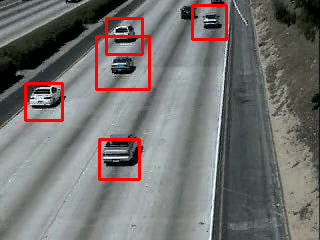
\includegraphics[width=\linewidth]{images/FinalOutput}}
  \caption{Image showing the detected vehicles sent back to local machine from the cloud VM}
\end{figure}

Other than this, we were also getting a warning "Gtk - Could not open display".  After some debugging, we found out that the reason for this error was that within the vehicle detection application, the algorithm was trying to create a new window.  As per our requirement, we didn't have any need to open a window and display the contents there.  Hence we simply removed this call that the algorithm made and instead added some other code due to which the image would be re-routed to the local host. 

Post these two changes, the application ran successfully on the clouds, carrying out all the processing on the remote VMs.  Once the required output file was created on the remote VM, it would create a directory on the host machine with the name as the floating IP address assigned earlier.  Within this directory, another directory named dev containing the vehicledetection folder was created.  The final image was placed within this vehicledetection folder.  Thus, as can be seen, ansible provides a robust and very secure way to access the systems (local as well as remote).  

\section{Benchmarking results and analysis}

For benchmarking, we first deployed the software stack onto the local
machine and then deployed it on the clouds.  We noted down the
observations in each case.  The parameters for benchmarking as well as
the observed values have been noted below.  In order to reduce any
errors, we have considered average values.  Thus, we installed each
software (from scratch) 3 times on the local machine and 3 times on
the clouds.  Then, we took the average of all these values in order to
find out the exact time needed for its deployment on the platform.

Also, for measuring the time, we used a shell script Setup.py.  This script displays the current time and then calls onto the Ansible playbook.  This Ansbile script then installs all the software on the software stack and then final comes to an end.  Once the Ansible script ends, the shell script again denotes the latest time.  The difference between these two timings displayed at the beginning and at the end give us the total software installation time required.  While testing it for different software, we had edited the playbook.yml file to contain only the single software under consideration.  In this way, we understood the time required for the installation of just a single software.  

\subsection{Deployment benchmarking}
Deployment benchmarking included observing the software deployment
times for each of the software in the software deployment stack.  We
started off with the first software, Git.  On the local machine, it
was installed in 2.57 seconds, while it took 10.45 seconds to be
installed on the clouds.  The next command, upgrade, took 35.84
seconds on the local machine and 155.03 seconds on the clouds.  Python
took 4.55 seconds to be installed on the local machine and 30.75
seconds to be installed on the clouds.  OpenCV, is a heavy software
having lots of dependencies on other software.  We thus had to
install it dependencies first before we could compile and install it.
Due to all this, OpenCV took 1420.37 to be installed on the clouds
and 276.01 seconds on the local machine.  Vehicle detection is a
lightweight application and as such, it took 11.99 to install on the
clouds and just 2.04 seconds to be installed on the local machine.
All these values have been tabulated in Table 1.

\begin{table}[]
\centering
\caption{Deployment Benchmark}
\label{Table 1}
\begin{tabular}{|l|l|l|}
\hline
 & Local VM avg time & Cloud VM avg time \\ \hline
Git & 2.59 & 10.49 \\ \hline
Upgrade & 35.53 & 155.59 \\ \hline
Python & 4.29 & 30.58 \\ \hline
OpenCV & 277.03 & 1419.53 \\ \hline
Vehicle Detection & 2.18 & 11.72 \\ \hline
\end{tabular}
\end{table}

\subsection{Elasticity benchmarking}
Elasticity metric aims to test the dependency of one software on the
other ones.  In other words, it aims to test a software's sensitivity
to changes in another software.  In our project, we noticed that some
of the software had a high dependency (and sensitivity), while others
had relatively low (or no) dependency.  For benchmarking the software
elasticity, we referred its ansible script.  We counted the number of
tasks that had to be successfully executed before the software in
question could be considered to be successfully installed.  For e.g.,
in case of the Vehicle Detection application, before running the
'make' command, we need to carry out 3 steps - getting the Vehicle
detection package source, changing the directory and running cmake.
Thus, the elasticity factor associated with the Vehicle Detection
project is 3.  We carried out a similar analysis of the other
software from the software stack.  Table 2 lists these observations.

\begin{table}[]
\centering
\caption{Elasticity benchmark}
\label{Table 2}
\begin{tabular}{|l|l|}
\hline
Software/Application & Dependency count \\ \hline
Git & 0 \\ \hline
Upgrade & NA \\ \hline
Python & 4 \\ \hline
OpenCV & 14 \\ \hline
Vehicle Detection & 3 \\ \hline
\end{tabular}
\end{table}

\subsection{Re-installation benchmarking}
Ansible scripts do a good job of installing the software.  However,
even before the software/applications are installed, ansible first
tests to make sure that the software is not already installed on the
system.  In case it is, then it simply skips over the installation
process of that software and then continues with the next one.  This
is important, since it does not try to update/reinstall the existing
software since that would lead to conflicts with the existing package
versions or features.  Also, since the re-installation of packages is
just skipped, in case of failures, there is no need to edit the
inventory.txt file to deploy only the failed software - it can be kept
as it is and the ansible scripts can be run from scratch.  Only the
failed software would be installed.  This also helps in reducing the
installation time.

\subsection{Workload benchmarking}
For Workload benchmarking, we found out the disk utilization of the
various software from the software stack.  While software such as
Git were pretty light, others like OpenCV were pretty heavy.  They not
only required a long time to install, but also consumed a lot of disk
space.  The output of the 'df -h' command on the cloud VMs has been shown.  We, thus, had used only 1.3 GB of
system space before installing OpenCV while we ended up consuming 4.4
GB of it after its installation.  The usage thus increased from 7
percent to 24 percent.

\begin{lstlisting}[
basicstyle=\footnotesize,
]
cc@abhinaik-011:~$ df -h
Filesystem                          Size  Used Avail Use% Mounted on
udev                                997M   12K  997M   1% /dev
tmpfs                               201M  340K  200M   1% /run
/dev/disk/by-label/                  20G  1.3G   18G   7% /
none                                4.0K     0  4.0K   0% /sys/fs/cgroup
none                                5.0M     0  5.0M   0% /run/lock
none                               1002M     0 1002M   0% /run/shm
none                                100M     0  100M   0% /run/user
\end{lstlisting}

\begin{lstlisting}[
basicstyle=\footnotesize,
]
cc@abhinaik-011:~$ df -h
Filesystem                          Size  Used Avail Use% Mounted on
udev                                997M   10M  987M   2% /dev
tmpfs                               201M  340K  200M   1% /run
/dev/disk/by-label/                  20G  4.4G   15G  24% /
none                                4.0K     0  4.0K   0% /sys/fs/cgroup
none                                5.0M     0  5.0M   0% /run/lock
none                               1002M     0 1002M   0% /run/shm
none                                100M     0  100M   0% /run/user
\end{lstlisting}

\subsection{Security and trust factors}
In our project we have used cloudmesh client which in turn uses the
SSH protocol to make secure connections to the VMs on the clouds
\cite{ssh-security}.  SSH is a cryptographic network protocol used for
establishing secured connections over the network.  It is thus used
for access to shell accounts on Unix like operating systems.  Since
SSH is being used, trustworthy connections can be established between
the local machine and the remote VMs on the clouds.  Along with this,
Ansible also helps in security enforcement.  Some of the qualities
like being agentless, capability to support SSH, no unnecessary
changes, modular structure, etc \cite{ansible-security}.

\subsection{Latency and reliability benchmarking}
We used the ping facility for benchmarking the latency
\cite{measuring-latency} of the network.  Latency measures the time it
takes for a packet to reach the cloud VM (with a specific IP) from the
local host.  We used the following command to test this:

\begin{lstlisting}
  ping 129.114.33.88 -c 10
\end{lstlisting}
	
In this command, the '-c 10' option makes 10 requests to the cloud
VMs.  In the end, it displays a summary of the results.  We can thus
observe that the minimum round trip time (rtt) was 43.729 seconds,
while the maximum was 45.216.  During one of the experiments, we noticed
that there was 10 percent packet loss, since out of the 10 packets
that were sent, only 9 of them could make it back to the local host.
However, repeated experiments showed that the system was indeed
reliable and that this was a small one-time exception.  

\begin{lstlisting}[
basicstyle=\small,
]
abhishek@abhishek:~$ ping 129.114.33.88 -c 10
PING 129.114.33.88 (129.114.33.88) 56(84) bytes of data.
64 bytes from 129.114.33.88: icmp_seq=1 ttl=51 time=45.2 ms
64 bytes from 129.114.33.88: icmp_seq=2 ttl=51 time=43.7 ms
64 bytes from 129.114.33.88: icmp_seq=3 ttl=51 time=43.8 ms
64 bytes from 129.114.33.88: icmp_seq=4 ttl=51 time=45.1 ms
64 bytes from 129.114.33.88: icmp_seq=5 ttl=51 time=44.6 ms
64 bytes from 129.114.33.88: icmp_seq=6 ttl=51 time=45.1 ms
64 bytes from 129.114.33.88: icmp_seq=7 ttl=51 time=44.2 ms
64 bytes from 129.114.33.88: icmp_seq=8 ttl=51 time=44.6 ms
64 bytes from 129.114.33.88: icmp_seq=9 ttl=51 time=44.3 ms
64 bytes from 129.114.33.88: icmp_seq=10 ttl=51 time=44.0 ms

--- 129.114.33.88 ping statistics ---
10 packets transmitted, 10 received, 0% packet loss, time 9012ms
rtt min/avg/max/mdev = 43.729/44.503/45.216/0.575 ms
\end{lstlisting}


\section{Conclusion}
In this project, we used cloudmesh client which is a client that
enables us to access and manage various cloud environments.  We used
it to gain access to Chameleon cloud VMs by using the SSH protocol.
Ansible is an automation platform that helps us in automating the
software deployment.  We used Ansible scripts to install all our
software along with the configuration of the project.  Once the
software stack was installed, we installed the Vehicle detection
application on top of it.  The Vehicle detection application running
on OpenCV used haar-classifiers to detect the vehicles.  It created an image wherein the vehicles were marked with a red rectangle.  This image, which was generated on the cloud, was then redirected to the local machine, using ansible fetch.  On the local machine, it was saved deep inside the directory named with the IP address.  Once this end-to-end process was
done, we did benchmarking of the system by using shell scripts.  We typically focused on the
deployment, elasticity, installation capacity, workload, security,
latency and reliability.

\section{Acknowledgments}
This project was undertaken as a part of the course objective for
I524: Big Data and Open Source Software Projects at Indiana
University, Bloomington.  We would like to thank Prof. Gregor Von
Laszewski and all the TAs for their help.  Similarly we would also
like to thank Andrews Sobral for providing us with the Vehicle
Detection application that we ran on the cloud VMs.

\bibliography{references}

\section*{Author Biographies}
\begingroup \setlength\intextsep{0pt}
\begin{minipage}[t][3.2cm][t]{1.0\columnwidth}
  \begin{wrapfigure}{L}{0.25\columnwidth}
    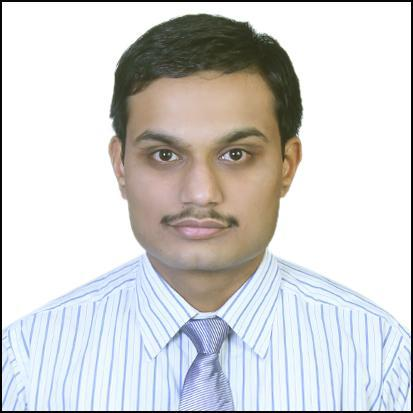
\includegraphics[width=0.25\columnwidth]{images/abhisheknaik.jpeg}
  \end{wrapfigure}
  \noindent
  {\bfseries Abhishek Naik} is a graduate student at Indiana
  University, Bloomington. He will receive his Masters degree in Computer Science in
  2018. His research interests include Big Data and Artificial Intelligence.
\end{minipage}
\begin{minipage}[t][3.2cm][t]{1.0\columnwidth}
  \begin{wrapfigure}{L}{0.25\columnwidth}
    
\includegraphics[width=0.25\columnwidth]{images/govindmishra.jpeg}
  \end{wrapfigure}
  \noindent
  {\bfseries Govind Mishra} is a graduate student at Indiana
  University, Bloomington. He will receive his Masters degree in Computer Science in 2018. His
  research interests include Big Data and Machine Learning.
\end{minipage}
\endgroup \appendix

\section{Work breakdown}
Abhishek Naik modified the Vehicle Detection application code so as to enable it to create a snapshot of the detected vehicles and save it as an image file.  This file was later re-routed back to the host machine.  He also wrote ansible scripts for the deployment of OpenCV, git and Vehicle Detection.  He also wrote the deployment, benchmarking and biography section of the report.\\
\\
Govind Mishra wrote down ansible scripts for the deployment of python and to carry out remote upgrade.  Besides this, we wrote down the introduction, requirements, software stack, execution, conclusion, acknowledgments, bibliography, biographies and the work breakdown sections of the report.

\end{document}
